\documentclass[10pt,letterpaper]{article}
\usepackage[utf8]{inputenc}
\usepackage{amsmath}
\usepackage{amsfonts}
\usepackage{amssymb}
\usepackage{graphicx}
\usepackage{wrapfig}
\usepackage{caption}
\usepackage{subcaption}
\usepackage[parfill]{parskip}
\usepackage[hidelinks]{hyperref}
\usepackage{verbatim}
\usepackage[left=2cm,right=2cm,top=2cm,bottom=2cm]{geometry}
\author{Kyle Colton \\ Thomas Kwak}
\title{Classification of Land Types Through Clustering}
\begin{document}
\maketitle

\section{Introduction}
\begin{wrapfigure}{r}{0.30\textwidth}
\begin{center}
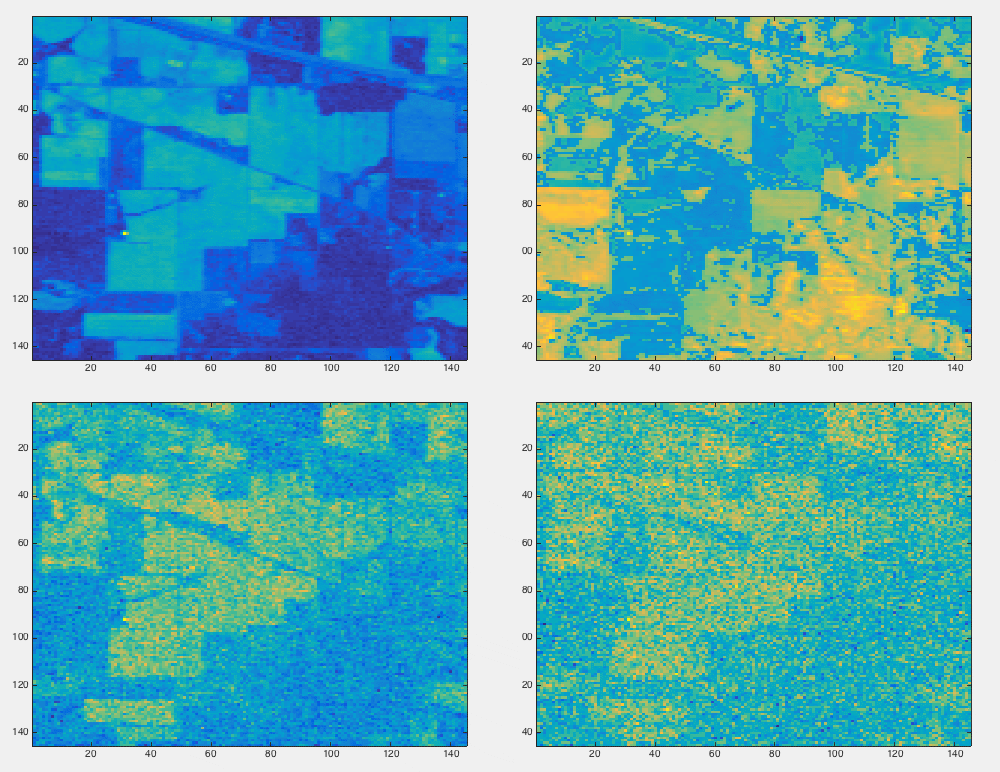
\includegraphics[width=.28\textwidth]{hyperSample.png}
\end{center}
\caption{Sample captures taken from the hyperspectral image}
\end{wrapfigure}
Hyperspectral imaging collects and processes information by taking images at varying frequencies within the EM spectrum. Because the imaging can divide the spectrum into more band than the human eye, hyperspectral imaging is used to find objects, identify materials, or detect certain processes. Therefore, there are multiple applications within the fields of astronomy, agriculture, biomedical imaging, physics, and geosciences.

One example of hyperspectral imaging is the Indian Pines test site in North-western Indiana. This dataset contains 145 by 145 pixel images taken at 224 different spectral reflectance bands in the wavelength ranging from 0.4 to 2.5 micrometers. Due to the region of water absorption, the number of bands had been reduced from 224 to 200.

The goals of this experiment are to use k-means clustering, soft-margin support vector machines, and linear models to separate and classify each pixel on the entire dataset set into one of the sixteen different crops found at the Indian Pines test site with accuracy as close as possible to the ground truth.
\section{Methods}
\subsection{K-Means Clustering}
K-means clustering is used to group samples into $k$ clusters such that the distances between the samples within each group is small compared to the distance between groups. This was used to group each of the pixels into either two, five, ten, or sixteen different groups.
\begin{figure}
\begin{center}
\begin{subfigure}[b]{0.24\textwidth}
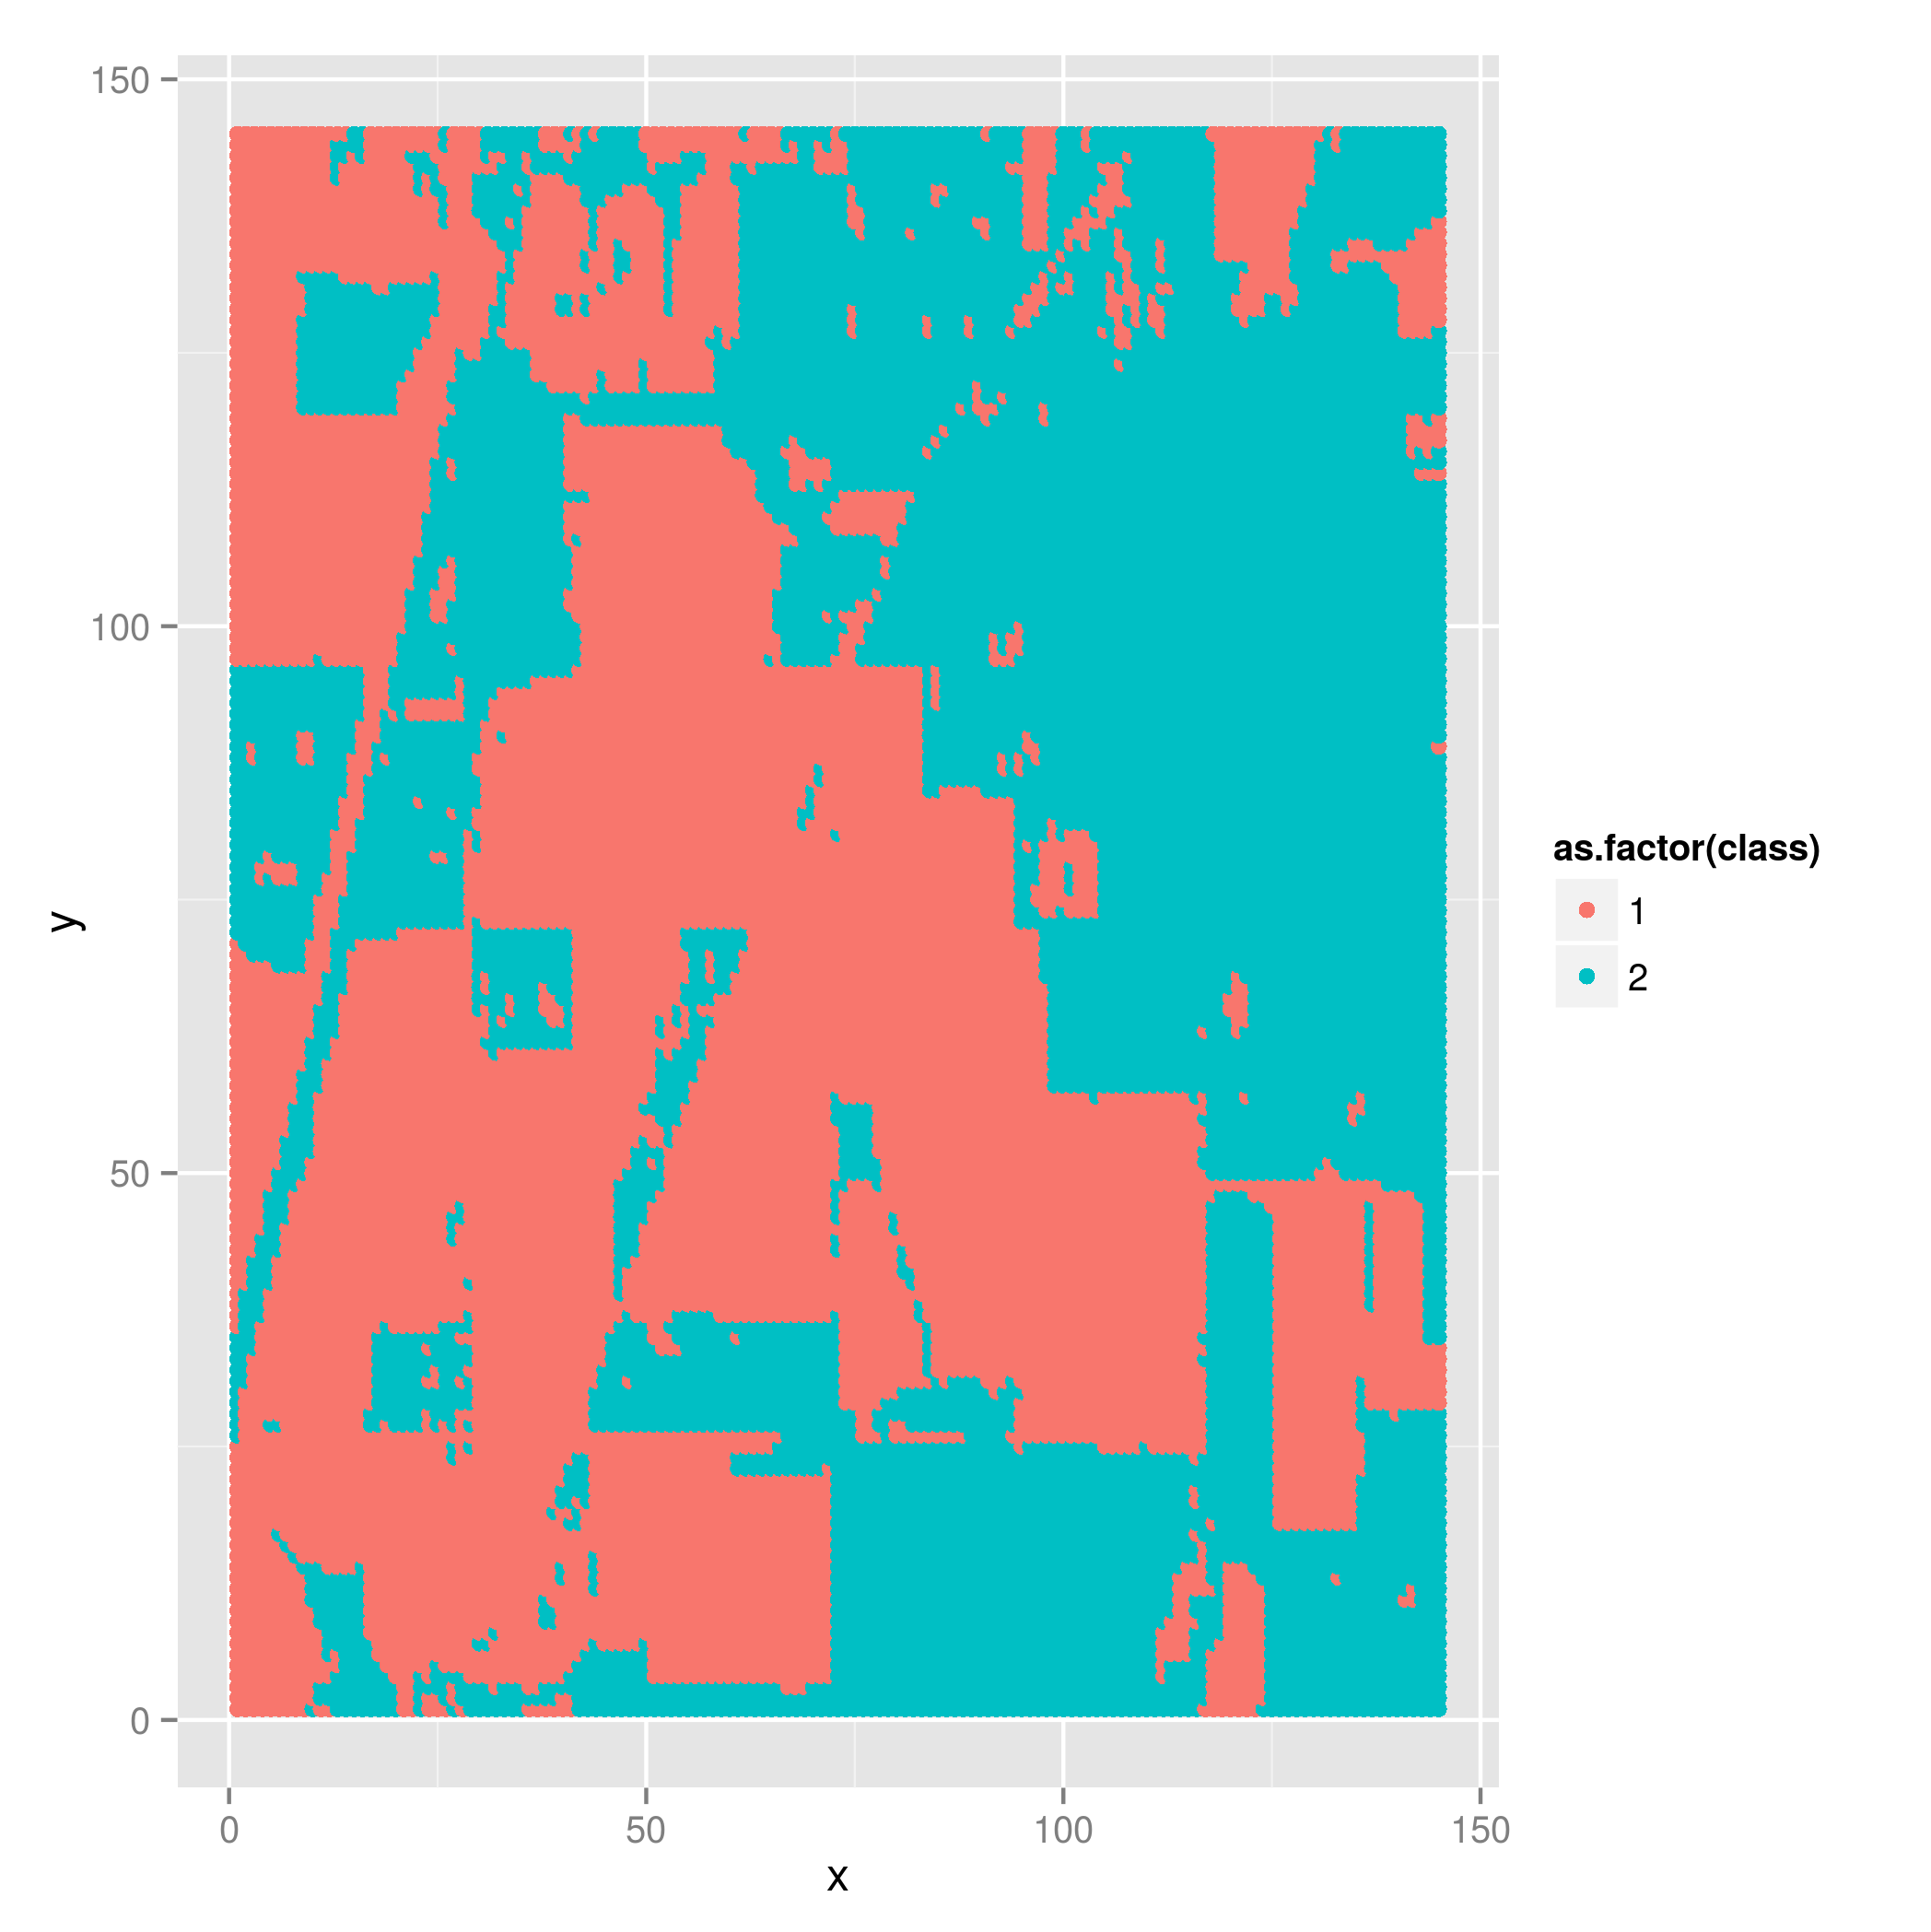
\includegraphics[width=\textwidth]{../Presentation/km2.png}
\caption{$k=2$}
\end{subfigure}
\begin{subfigure}[b]{0.24\textwidth}
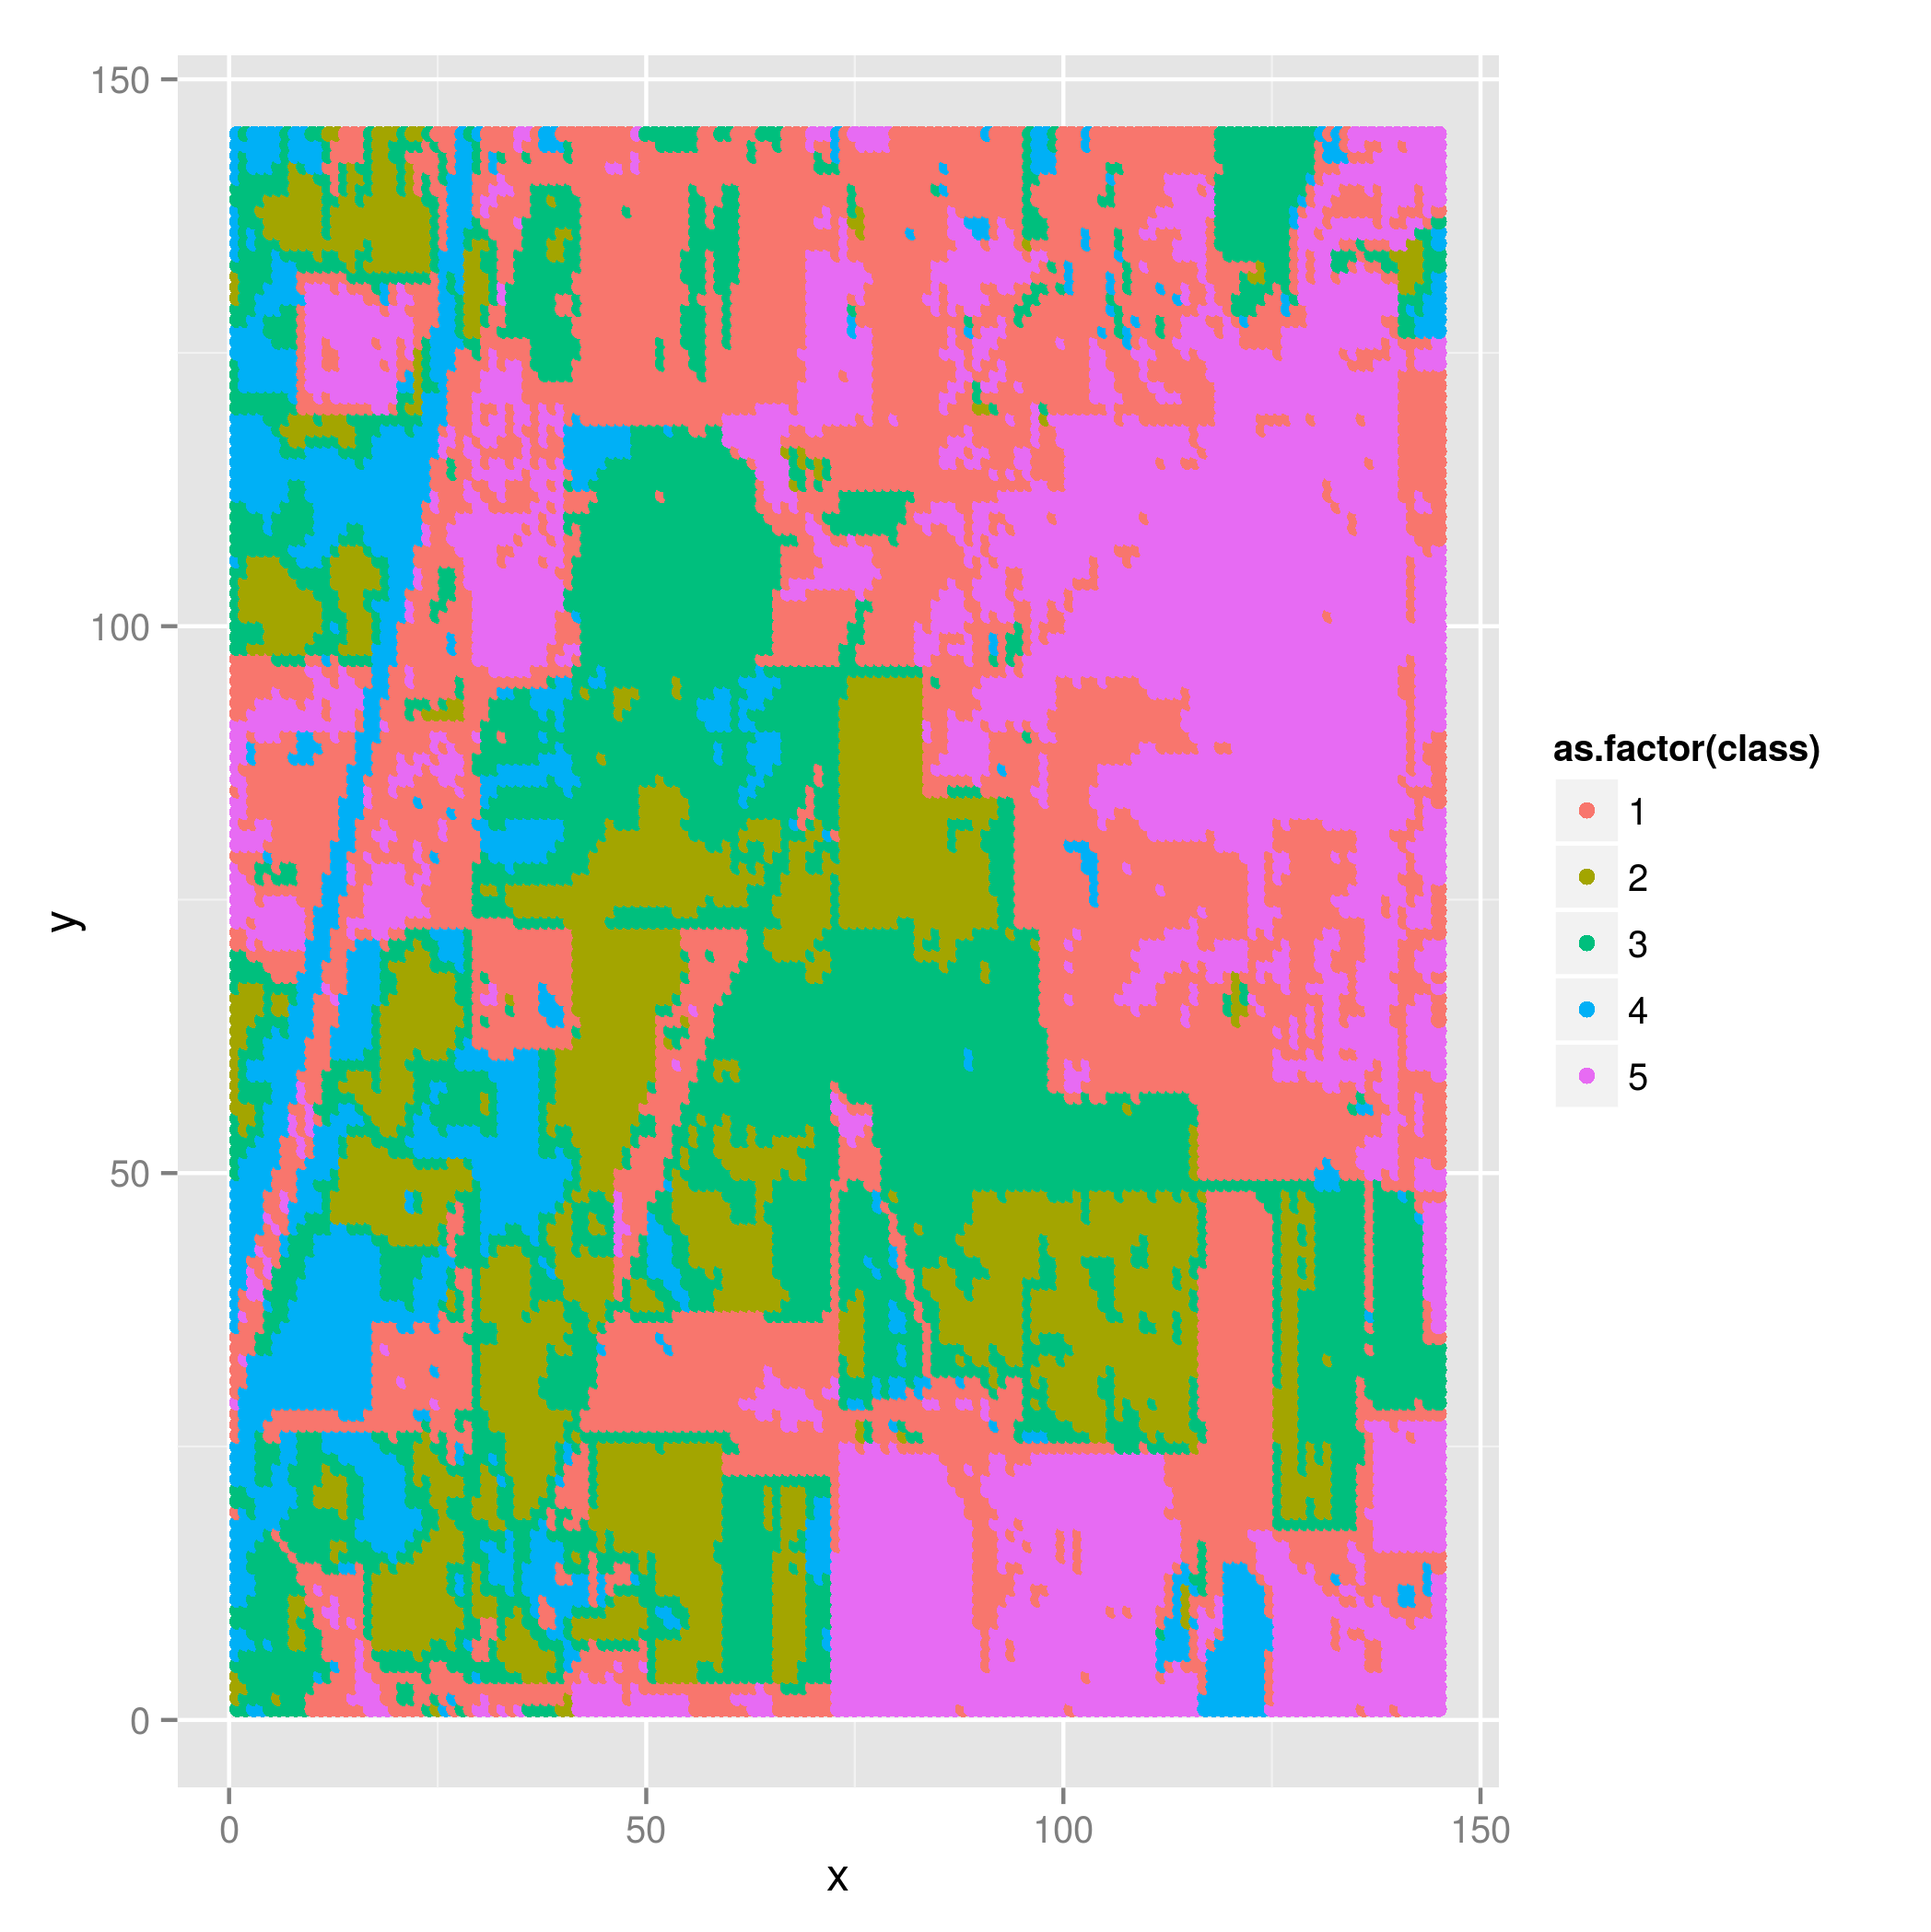
\includegraphics[width=\textwidth]{../Presentation/km5.png}
\caption{$k=5$}
\end{subfigure}
\begin{subfigure}[b]{0.24\textwidth}
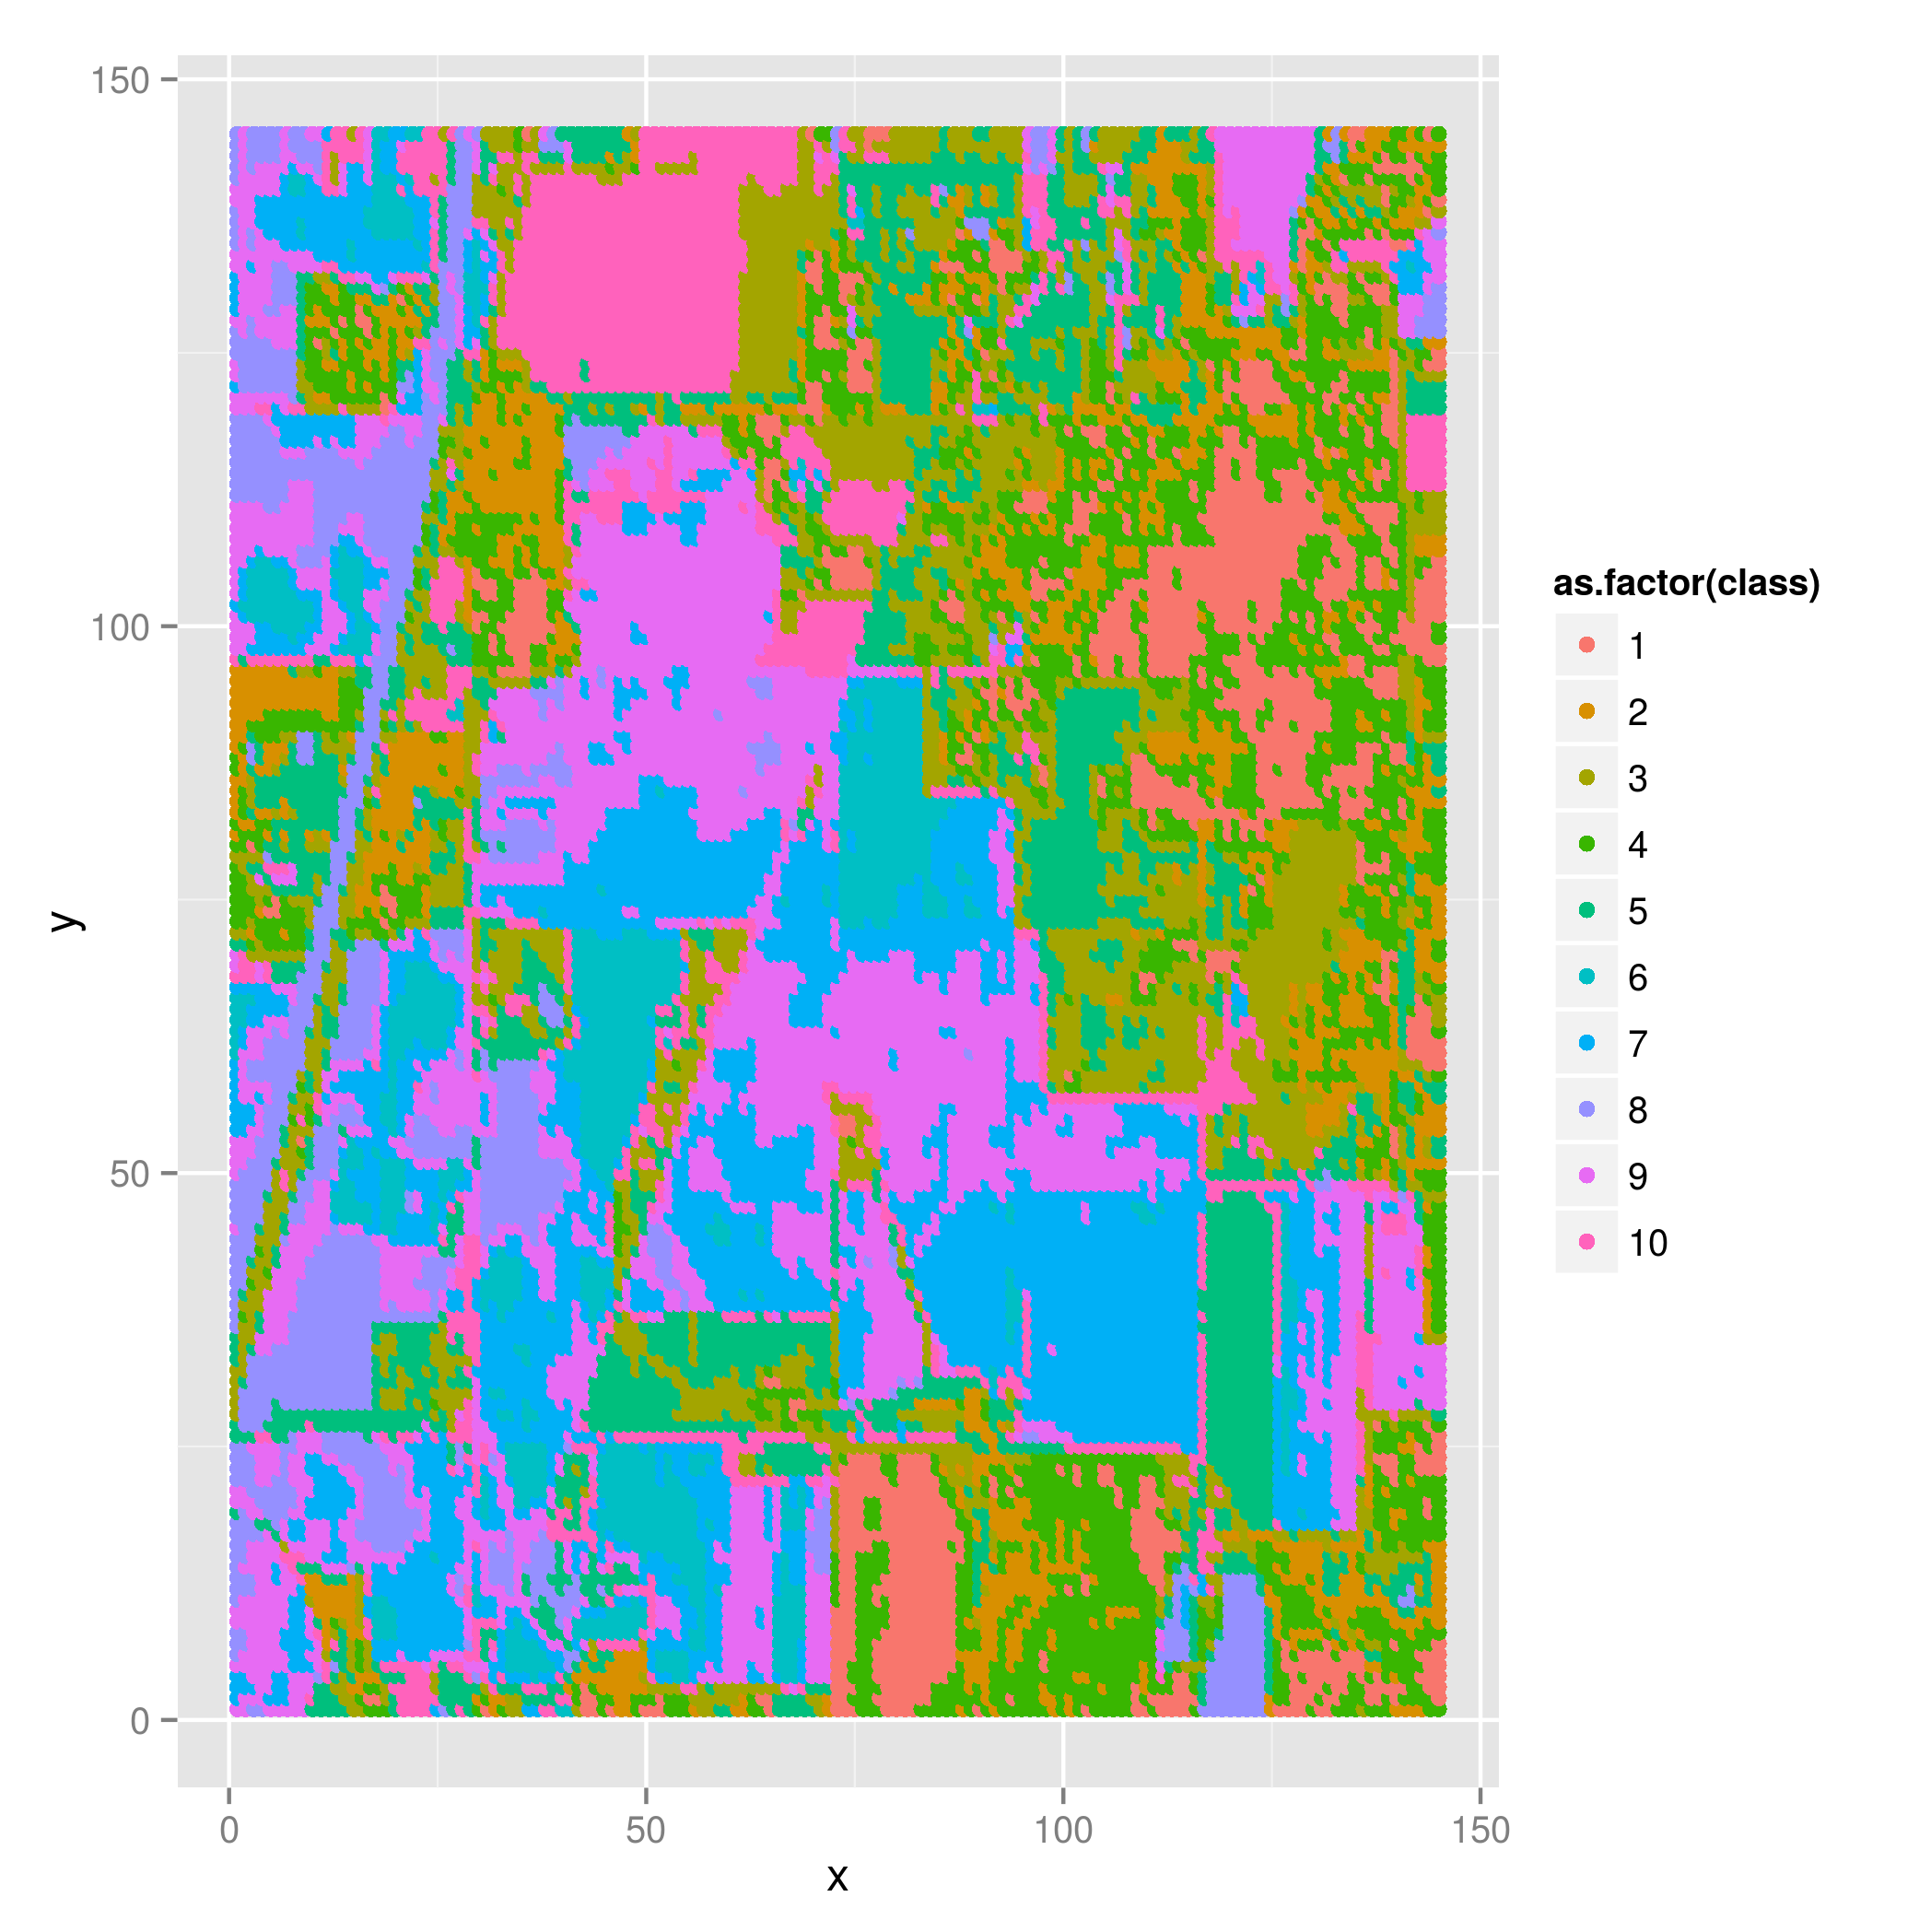
\includegraphics[width=\textwidth]{../Presentation/km10.png}
\caption{$k=10$}
\end{subfigure}
\begin{subfigure}[b]{0.24\textwidth}
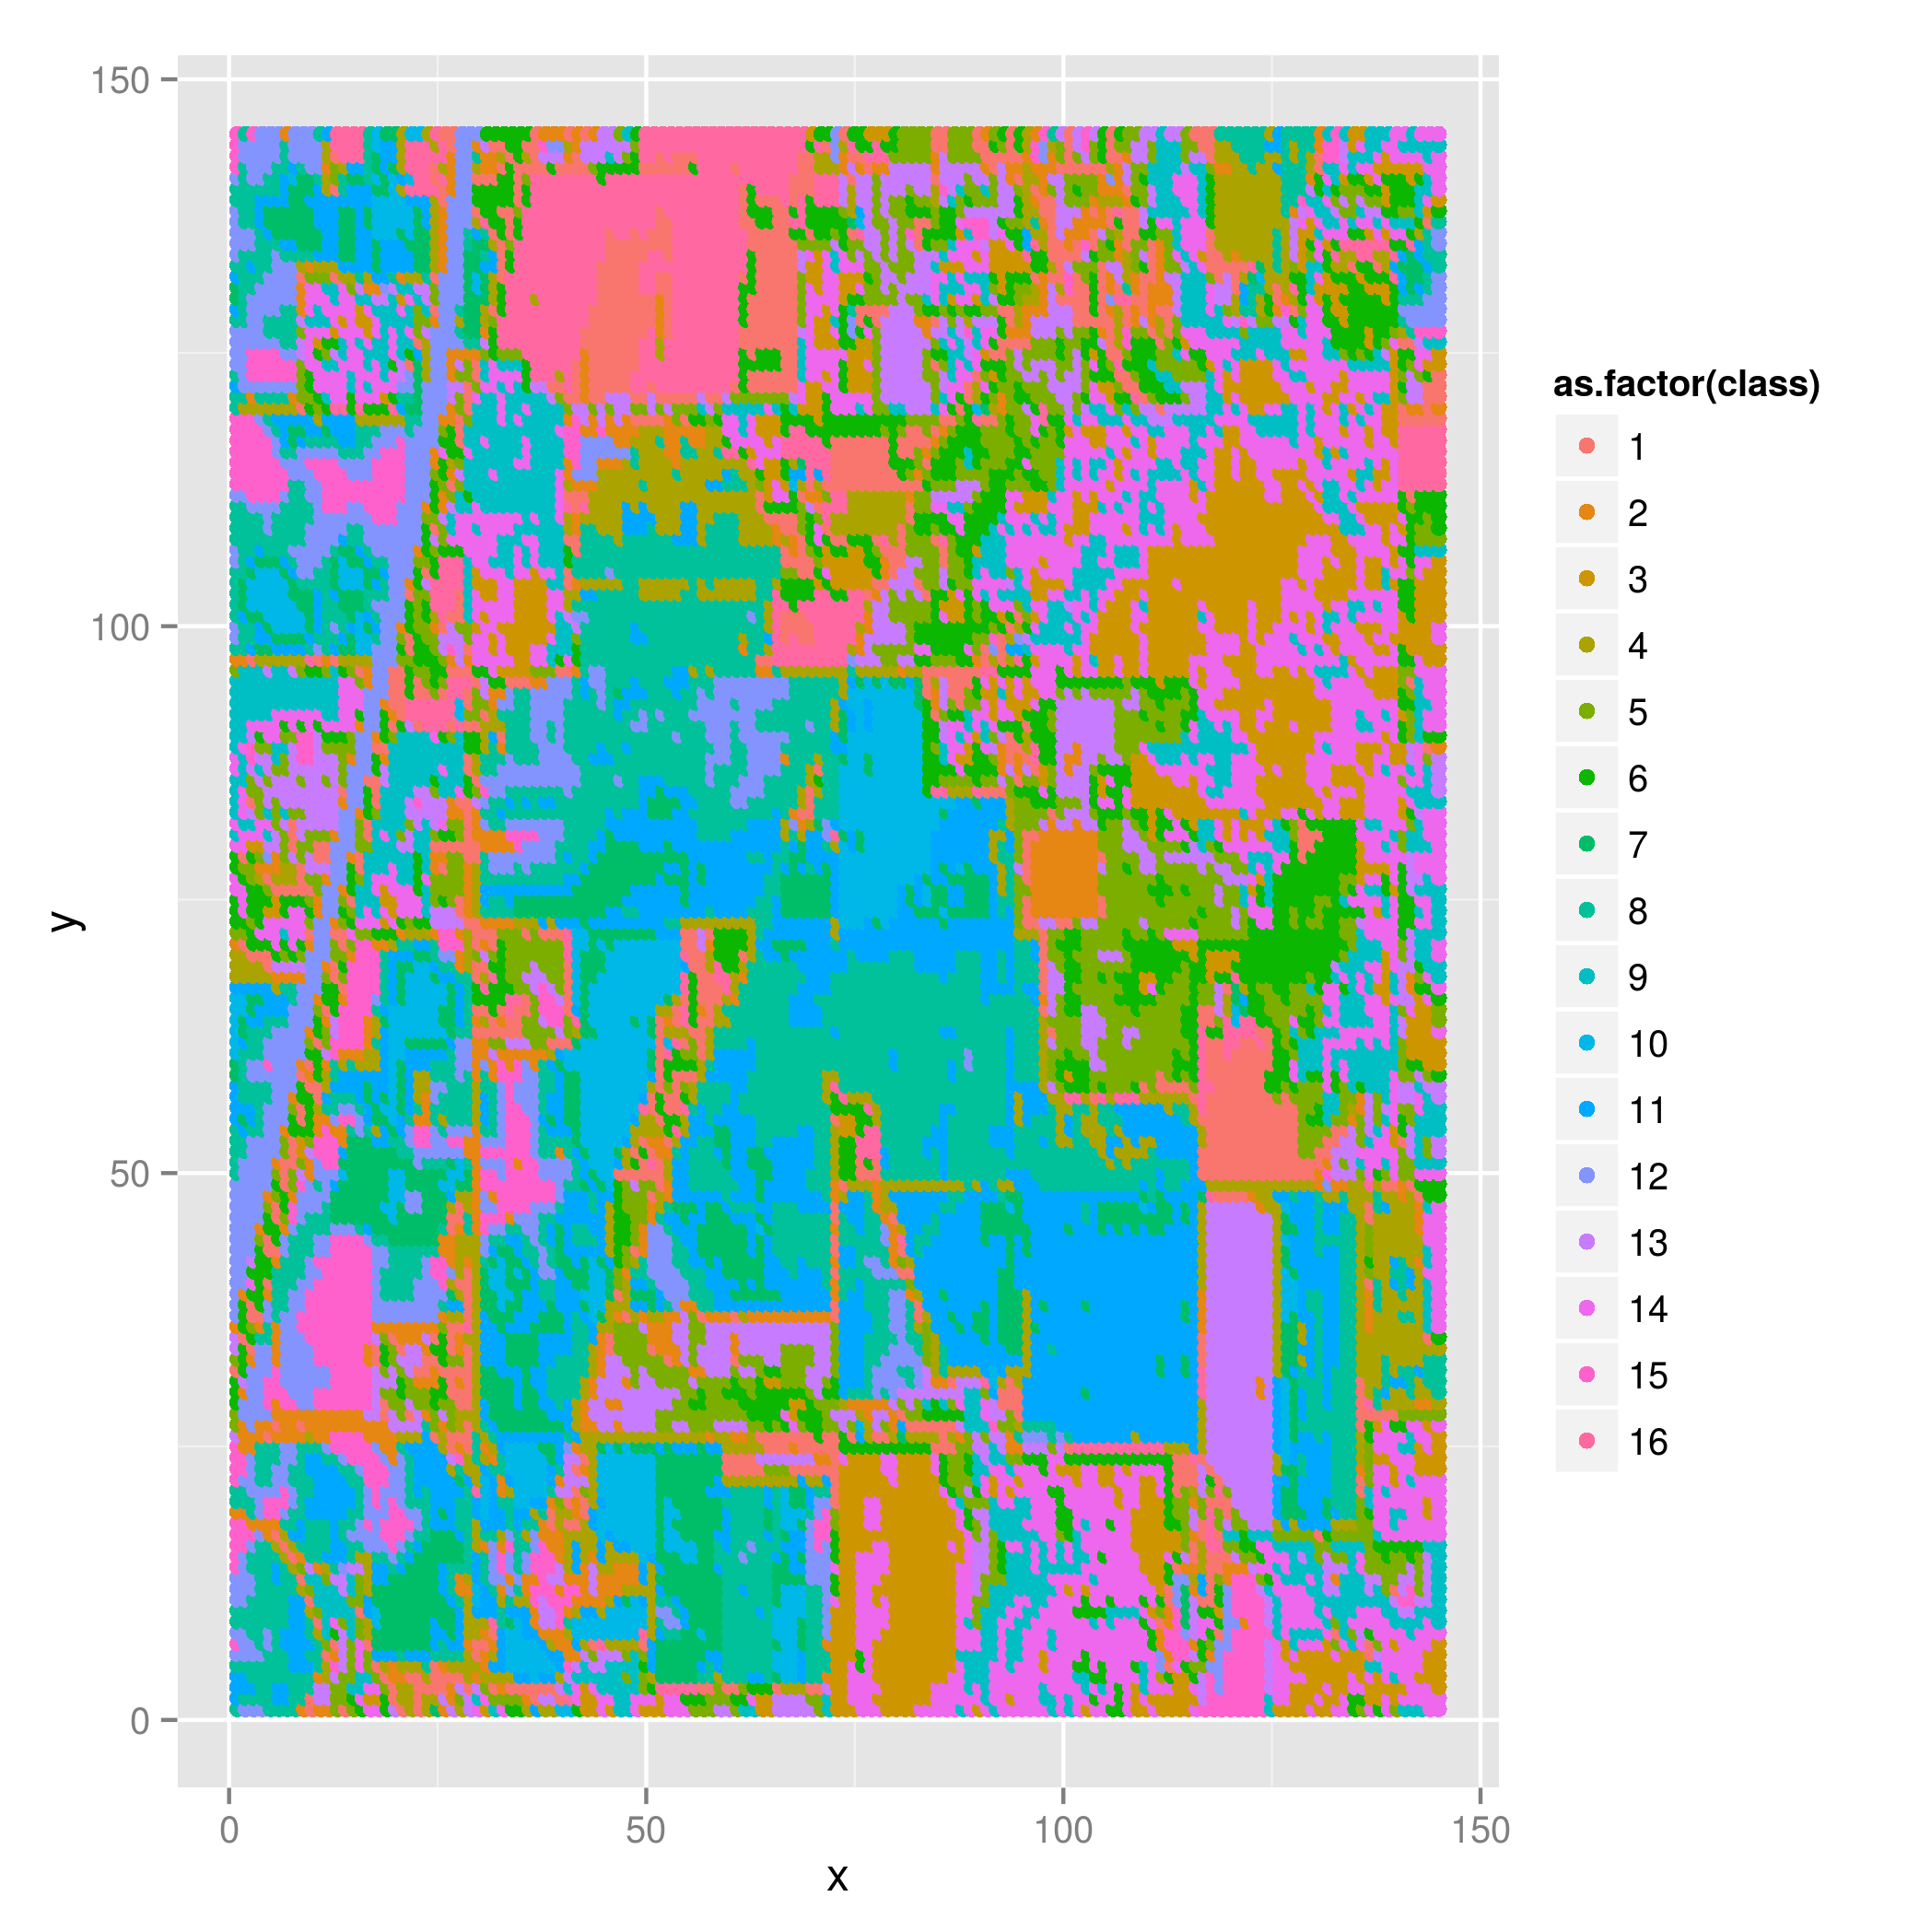
\includegraphics[width=\textwidth]{../Presentation/km16.png}
\caption{$k=16$}
\end{subfigure}
\caption{K Means at various values of $k$ clusters}
\end{center}
\end{figure}
\subsection{Soft-Margin Support Vector Machines}
Soft-margin support vector machines are supervised learning models used for classification through pattern recognition. Soft-margin support vector machines were used instead of hard-margin support vector machines because the dataset was found to be not linearly separable. A quarter of the ground truth dataset was used as training data for the soft-margin multiclass support vector machine.
\subsection{Principle Component Analysis}
To reduce the size of the dataset, principal component analysis was used on the data set after concatenating all bands into a single matrix. This method can then reduce the dataset into the necessary principal components, thus reducing the size of the overall dataset. By comparing the unweighted and weighted principal components, there is a reduction in preprocessing data from 21025 dimensions to 200 dimensions without much loss in accuracy.
\section{Results}
\subsection{K-Means Clustering}
As the number of classes increased, more landtypes were able to be distinguished. However, the level of noise also increased as the number of classes increased. While K-Means was able to get general shapes, the individual crop-detection was noisy.
\subsection{Soft-Margin Support Vector machines}
\begin{wrapfigure}{r}{0.3\textwidth}\vspace{-20pt}
\begin{center}
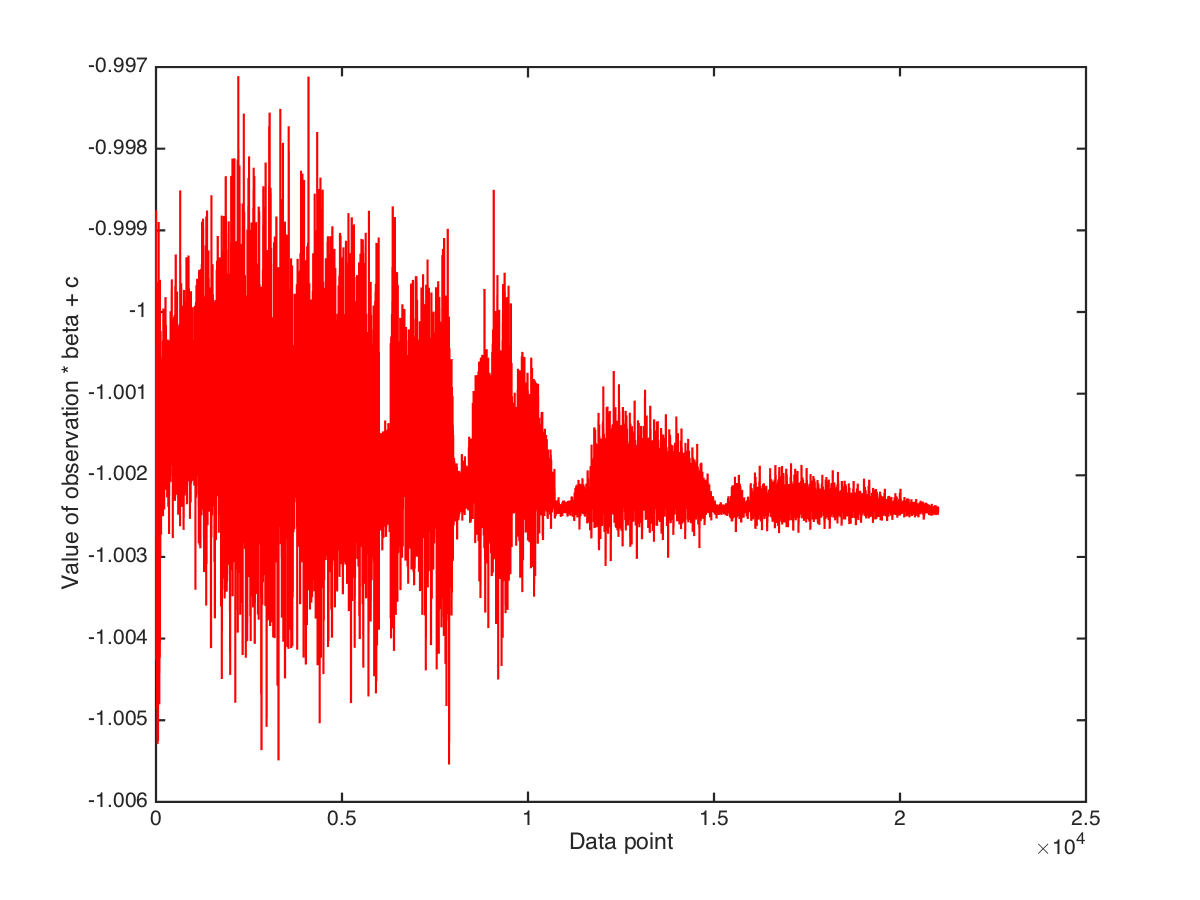
\includegraphics[width=0.28\textwidth, height=80pt]{../Presentation/softsvmImage.png}
\caption{Testing linear separability using SVM}
\end{center}
\end{wrapfigure}
Initially, simple SVM was run to test the separability of the data into two classes. The data was found to be not linearly separable.

Multiple SVM was used from the R library \texttt{e1071}. While simple SVM allows for 2 class selection, the multiclass SVM allows a greater number of classes by running SVM multiple times. A cost analysis was run to see the performance of the model as a function of cost. The maximum accuracy found by the soft-margin SVM was approximately 83.5\% at a constraint violation cost of 100. Generally, model accuracy increased as constraint violation cost increased.

Multiclass SVM was done using the gaussian radial basis kernel.
\begin{figure}[!hb]
\begin{center}
\begin{subfigure}[b]{0.3\textwidth}
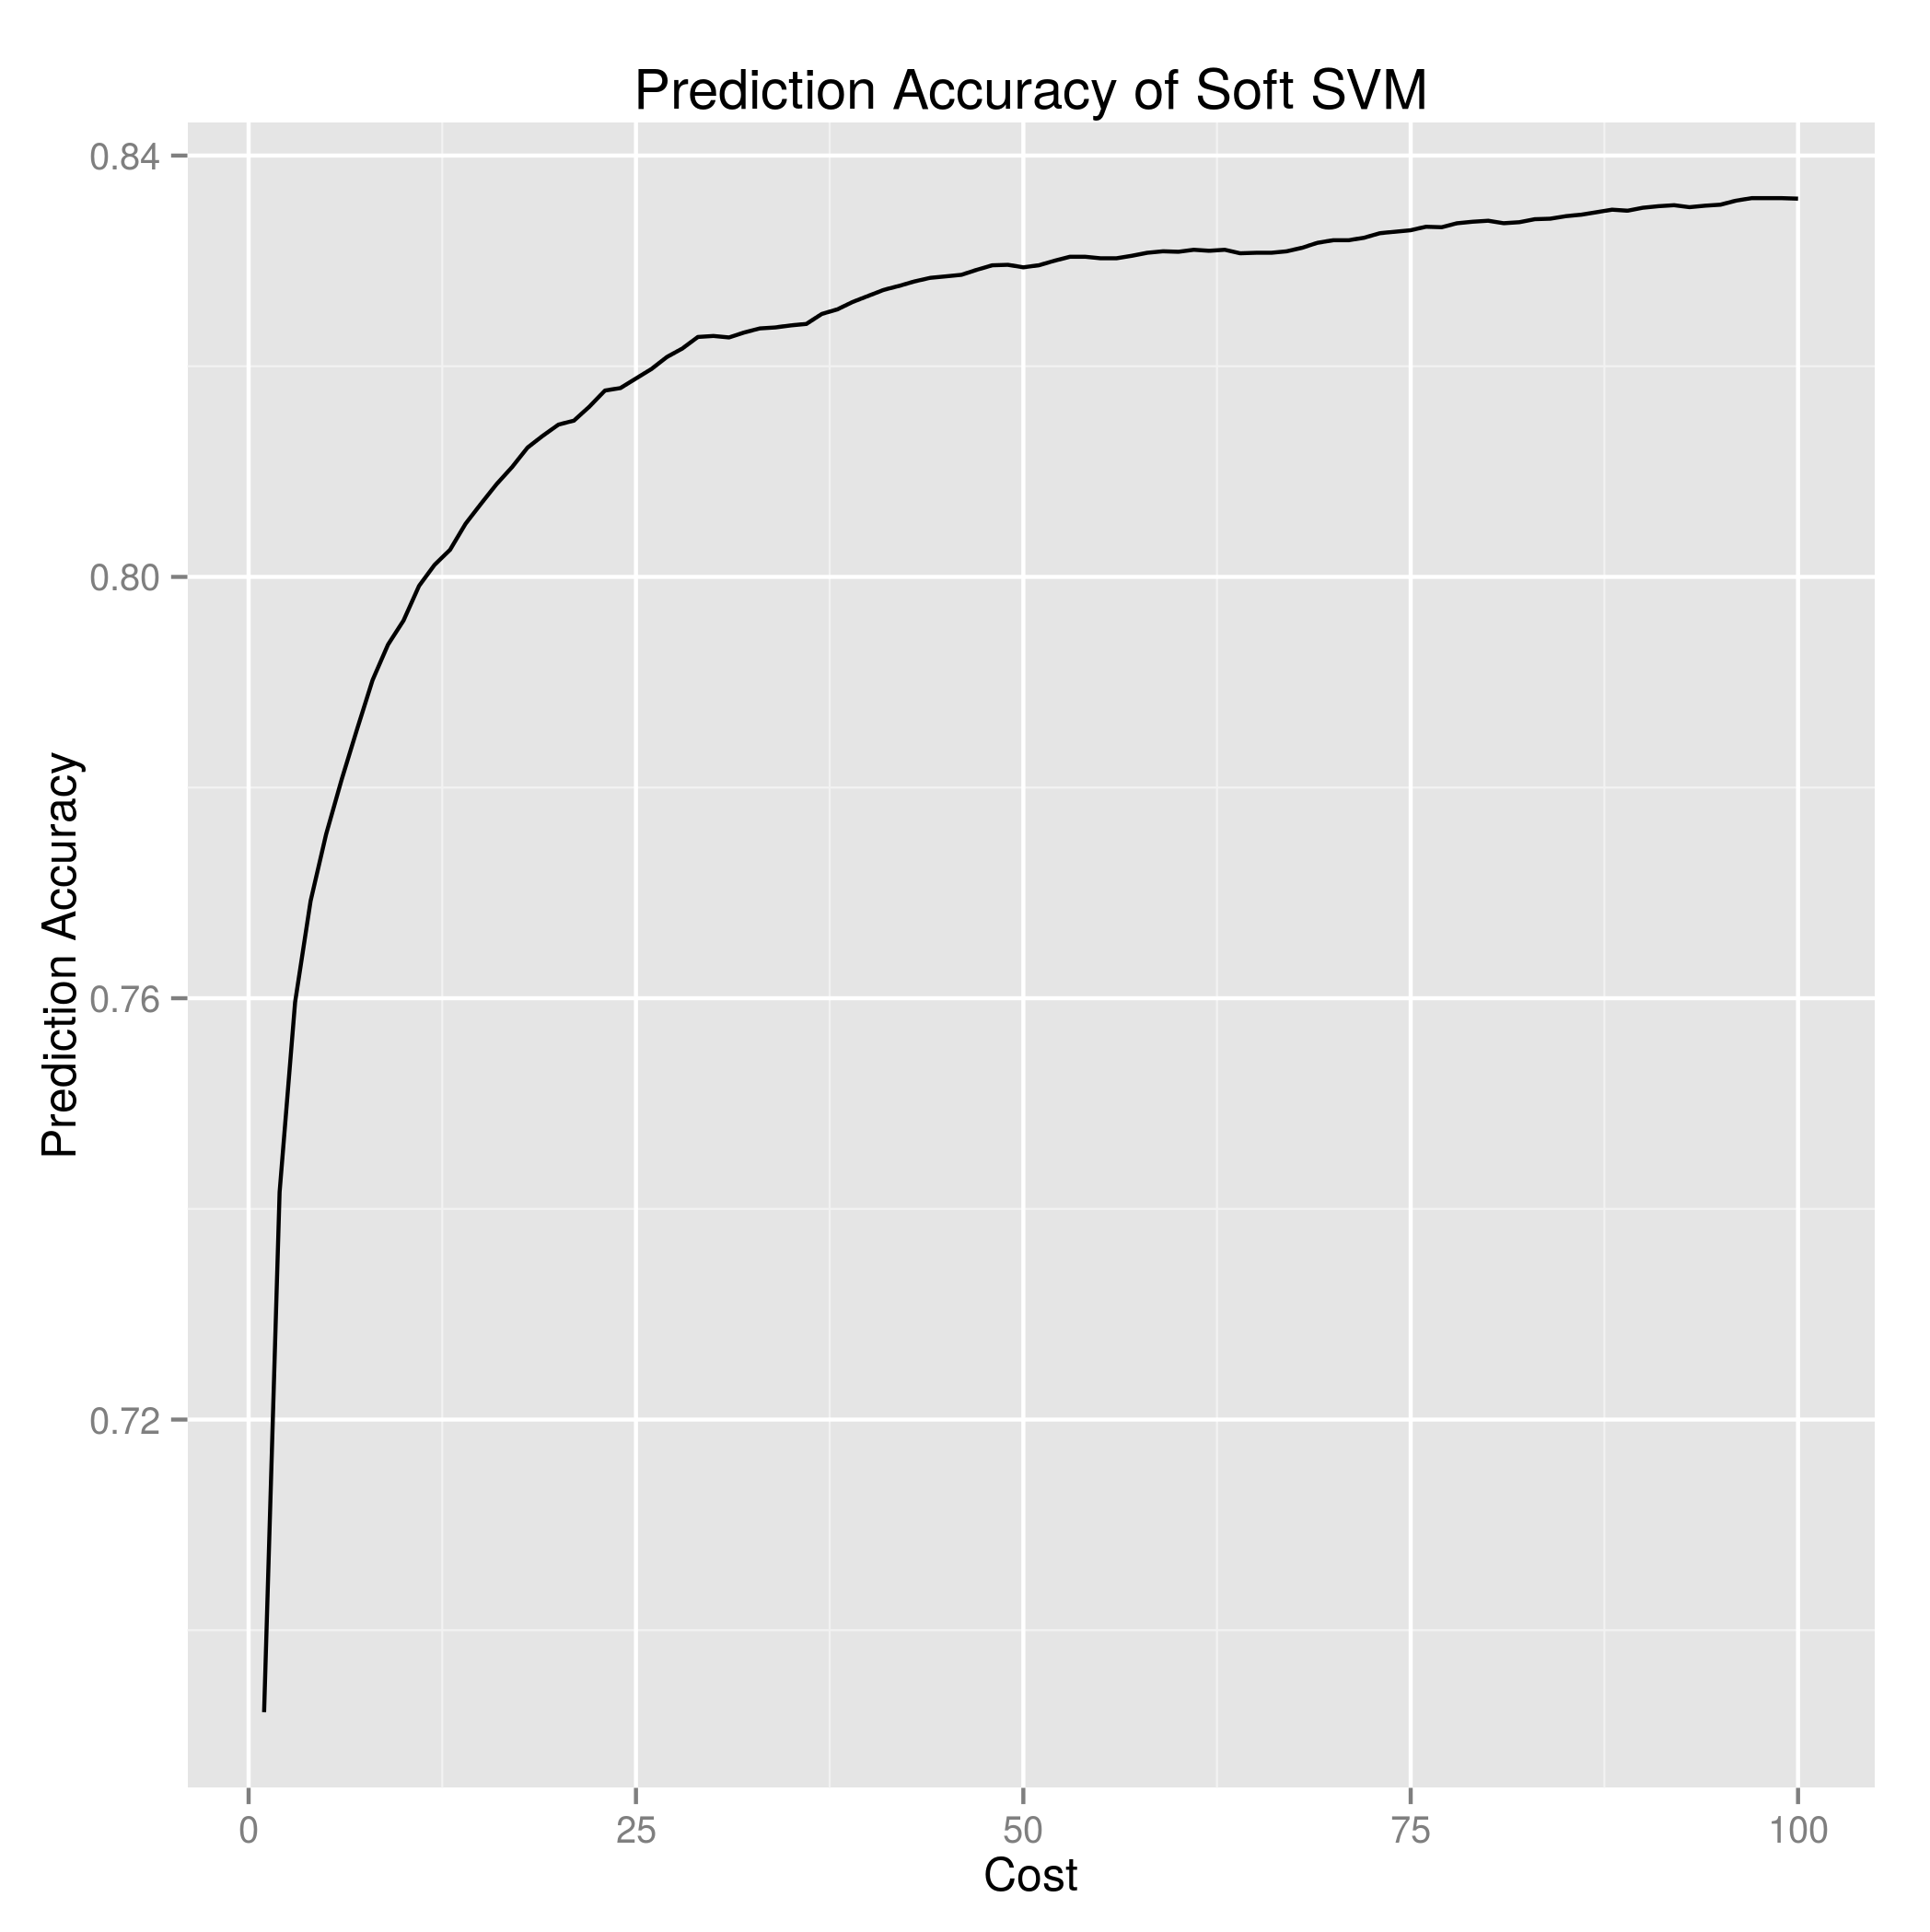
\includegraphics[width=\textwidth]{SVM_accuracy.png}
\caption{SVM Accuracy vs Cost}
\end{subfigure}
\begin{subfigure}[b]{0.3\textwidth}
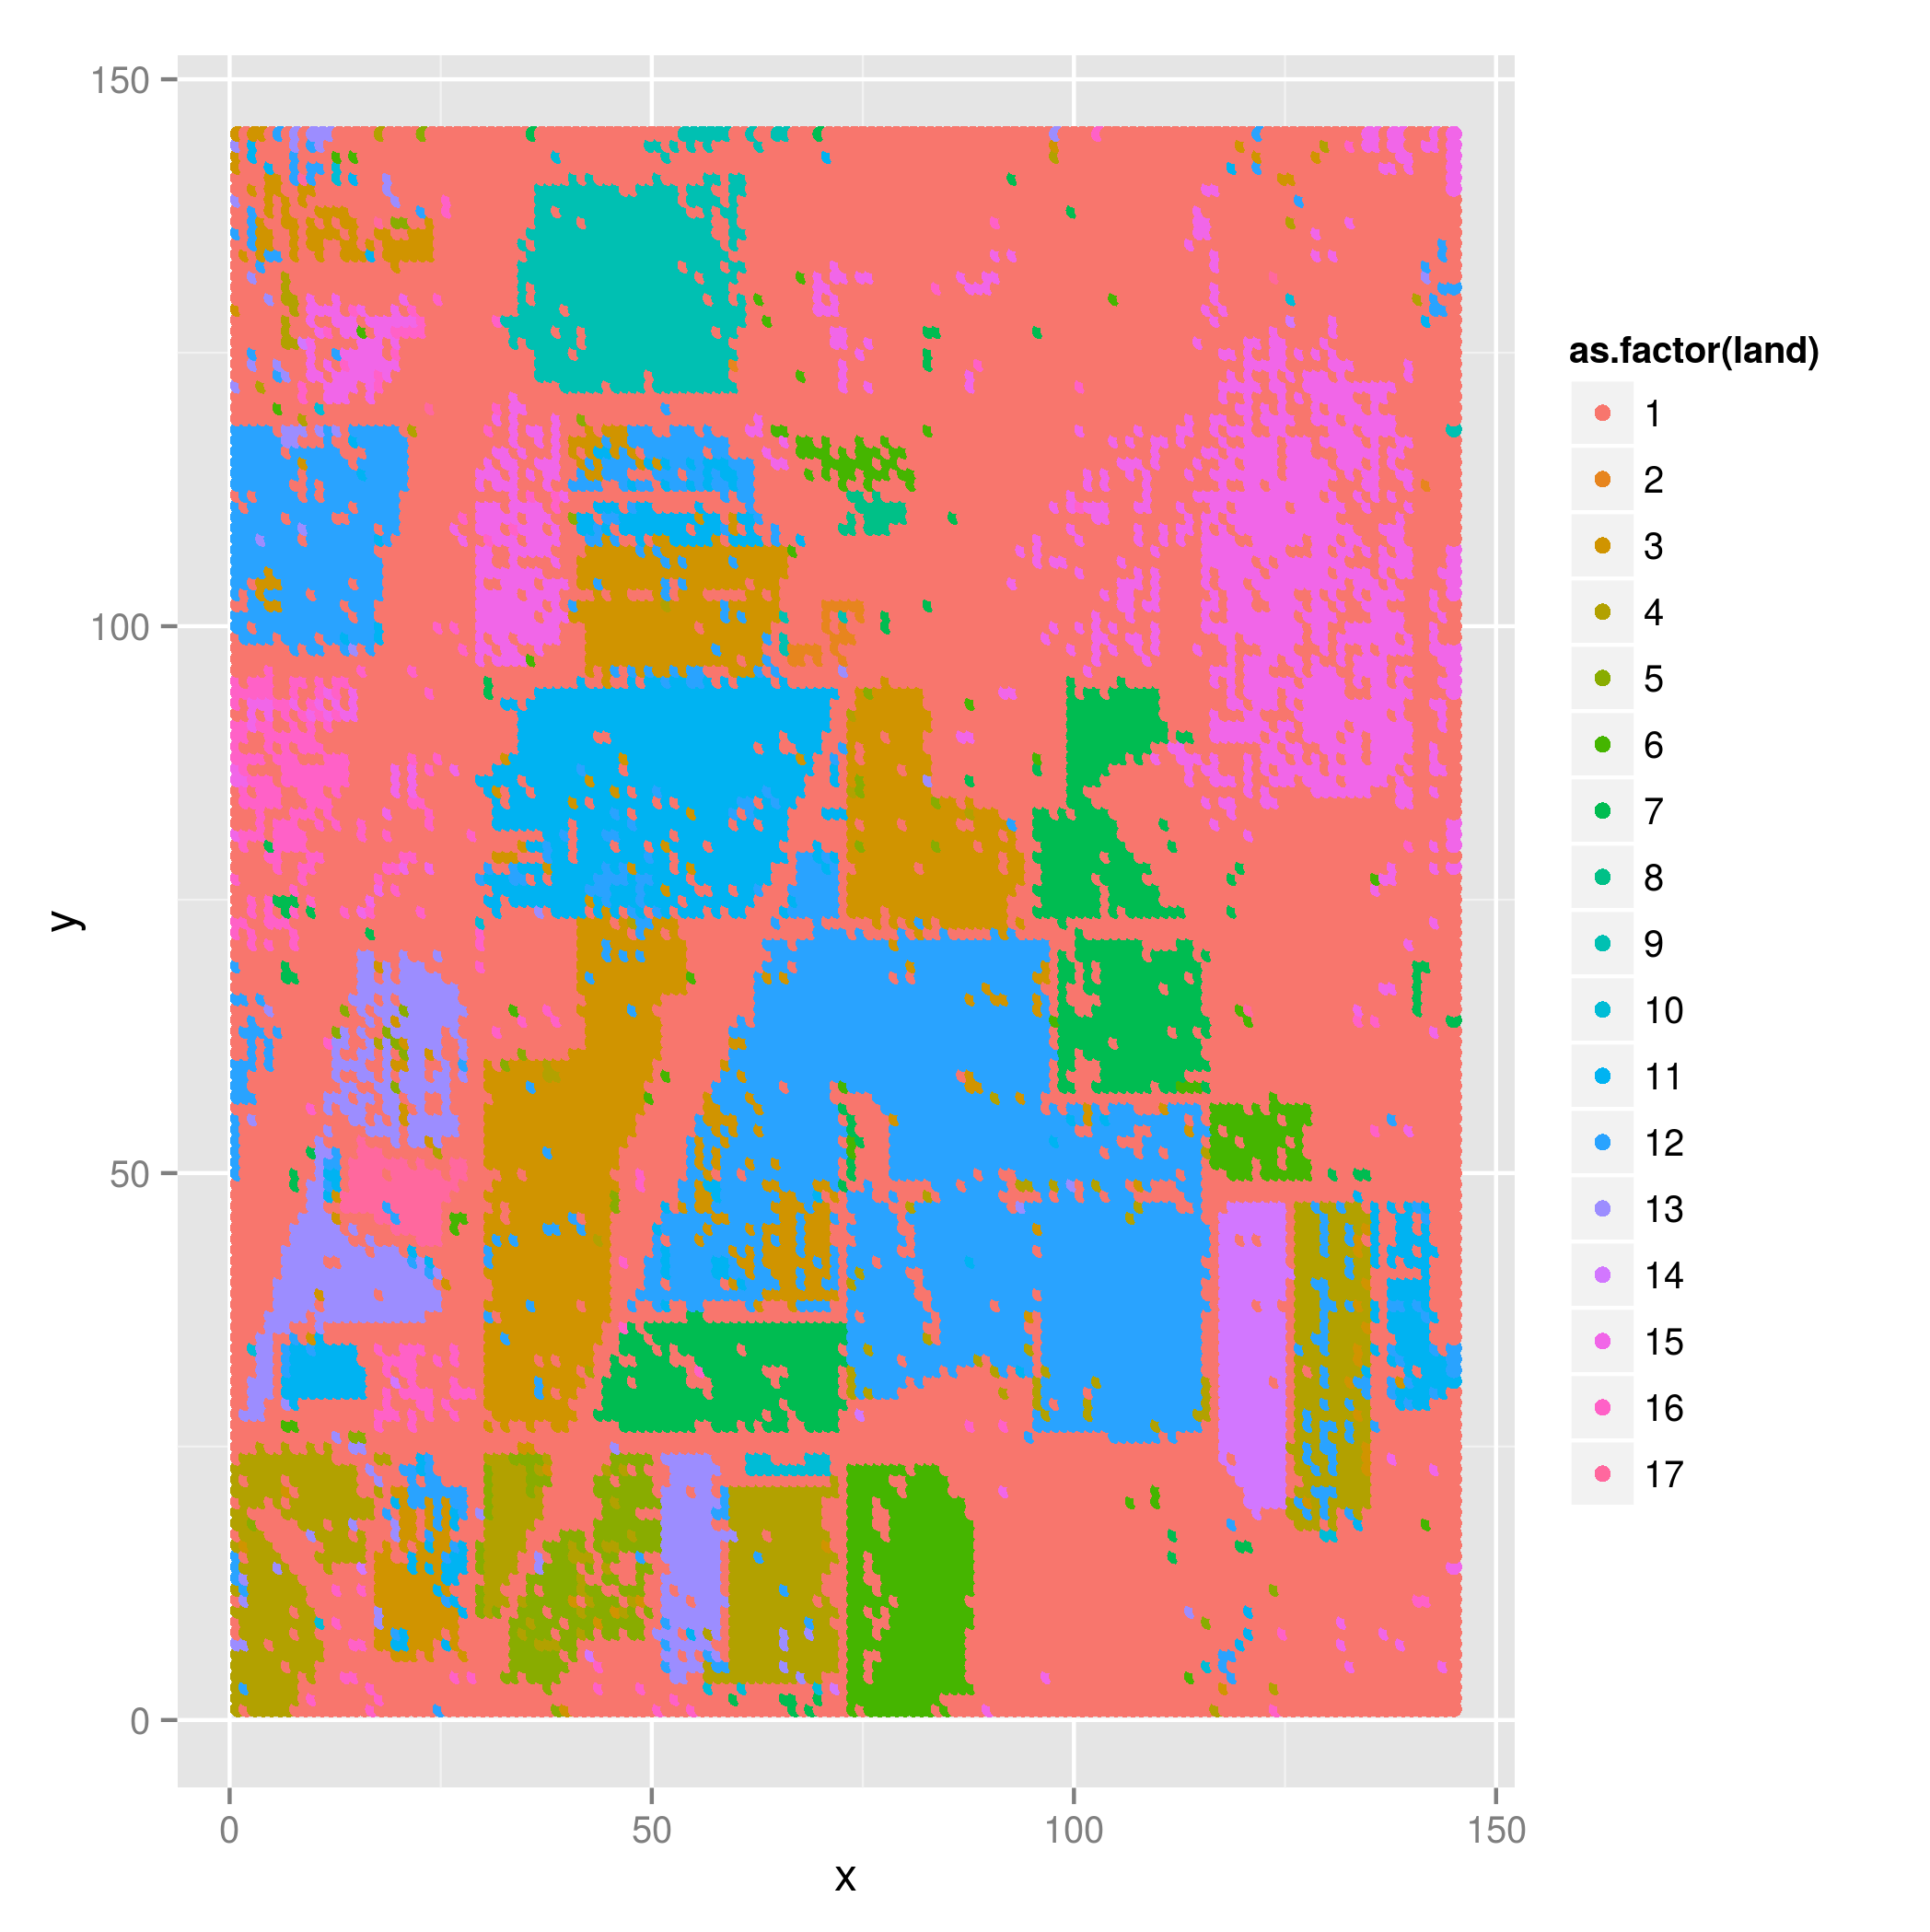
\includegraphics[width=\textwidth]{SVM_Landtypes.png}
\caption{SVM Classification Map}
\end{subfigure}
\caption{Multiple SVM}
\end{center}
\end{figure}
\subsection{Principle Component Analysis}
Using PCA, the dataset was reduced from a 200 x 21025 matrix to a 200 x 200 matrix. From the unweighted PCA, approximately 93.5\% of the variance could be explained by just the first three principal components. From the weighted PCA, approximately 90.4\% of the variance could be explained by the first three principal components.
\section{Discussion}
\begin{wrapfigure}{r}{0.4\textwidth}
\begin{center}
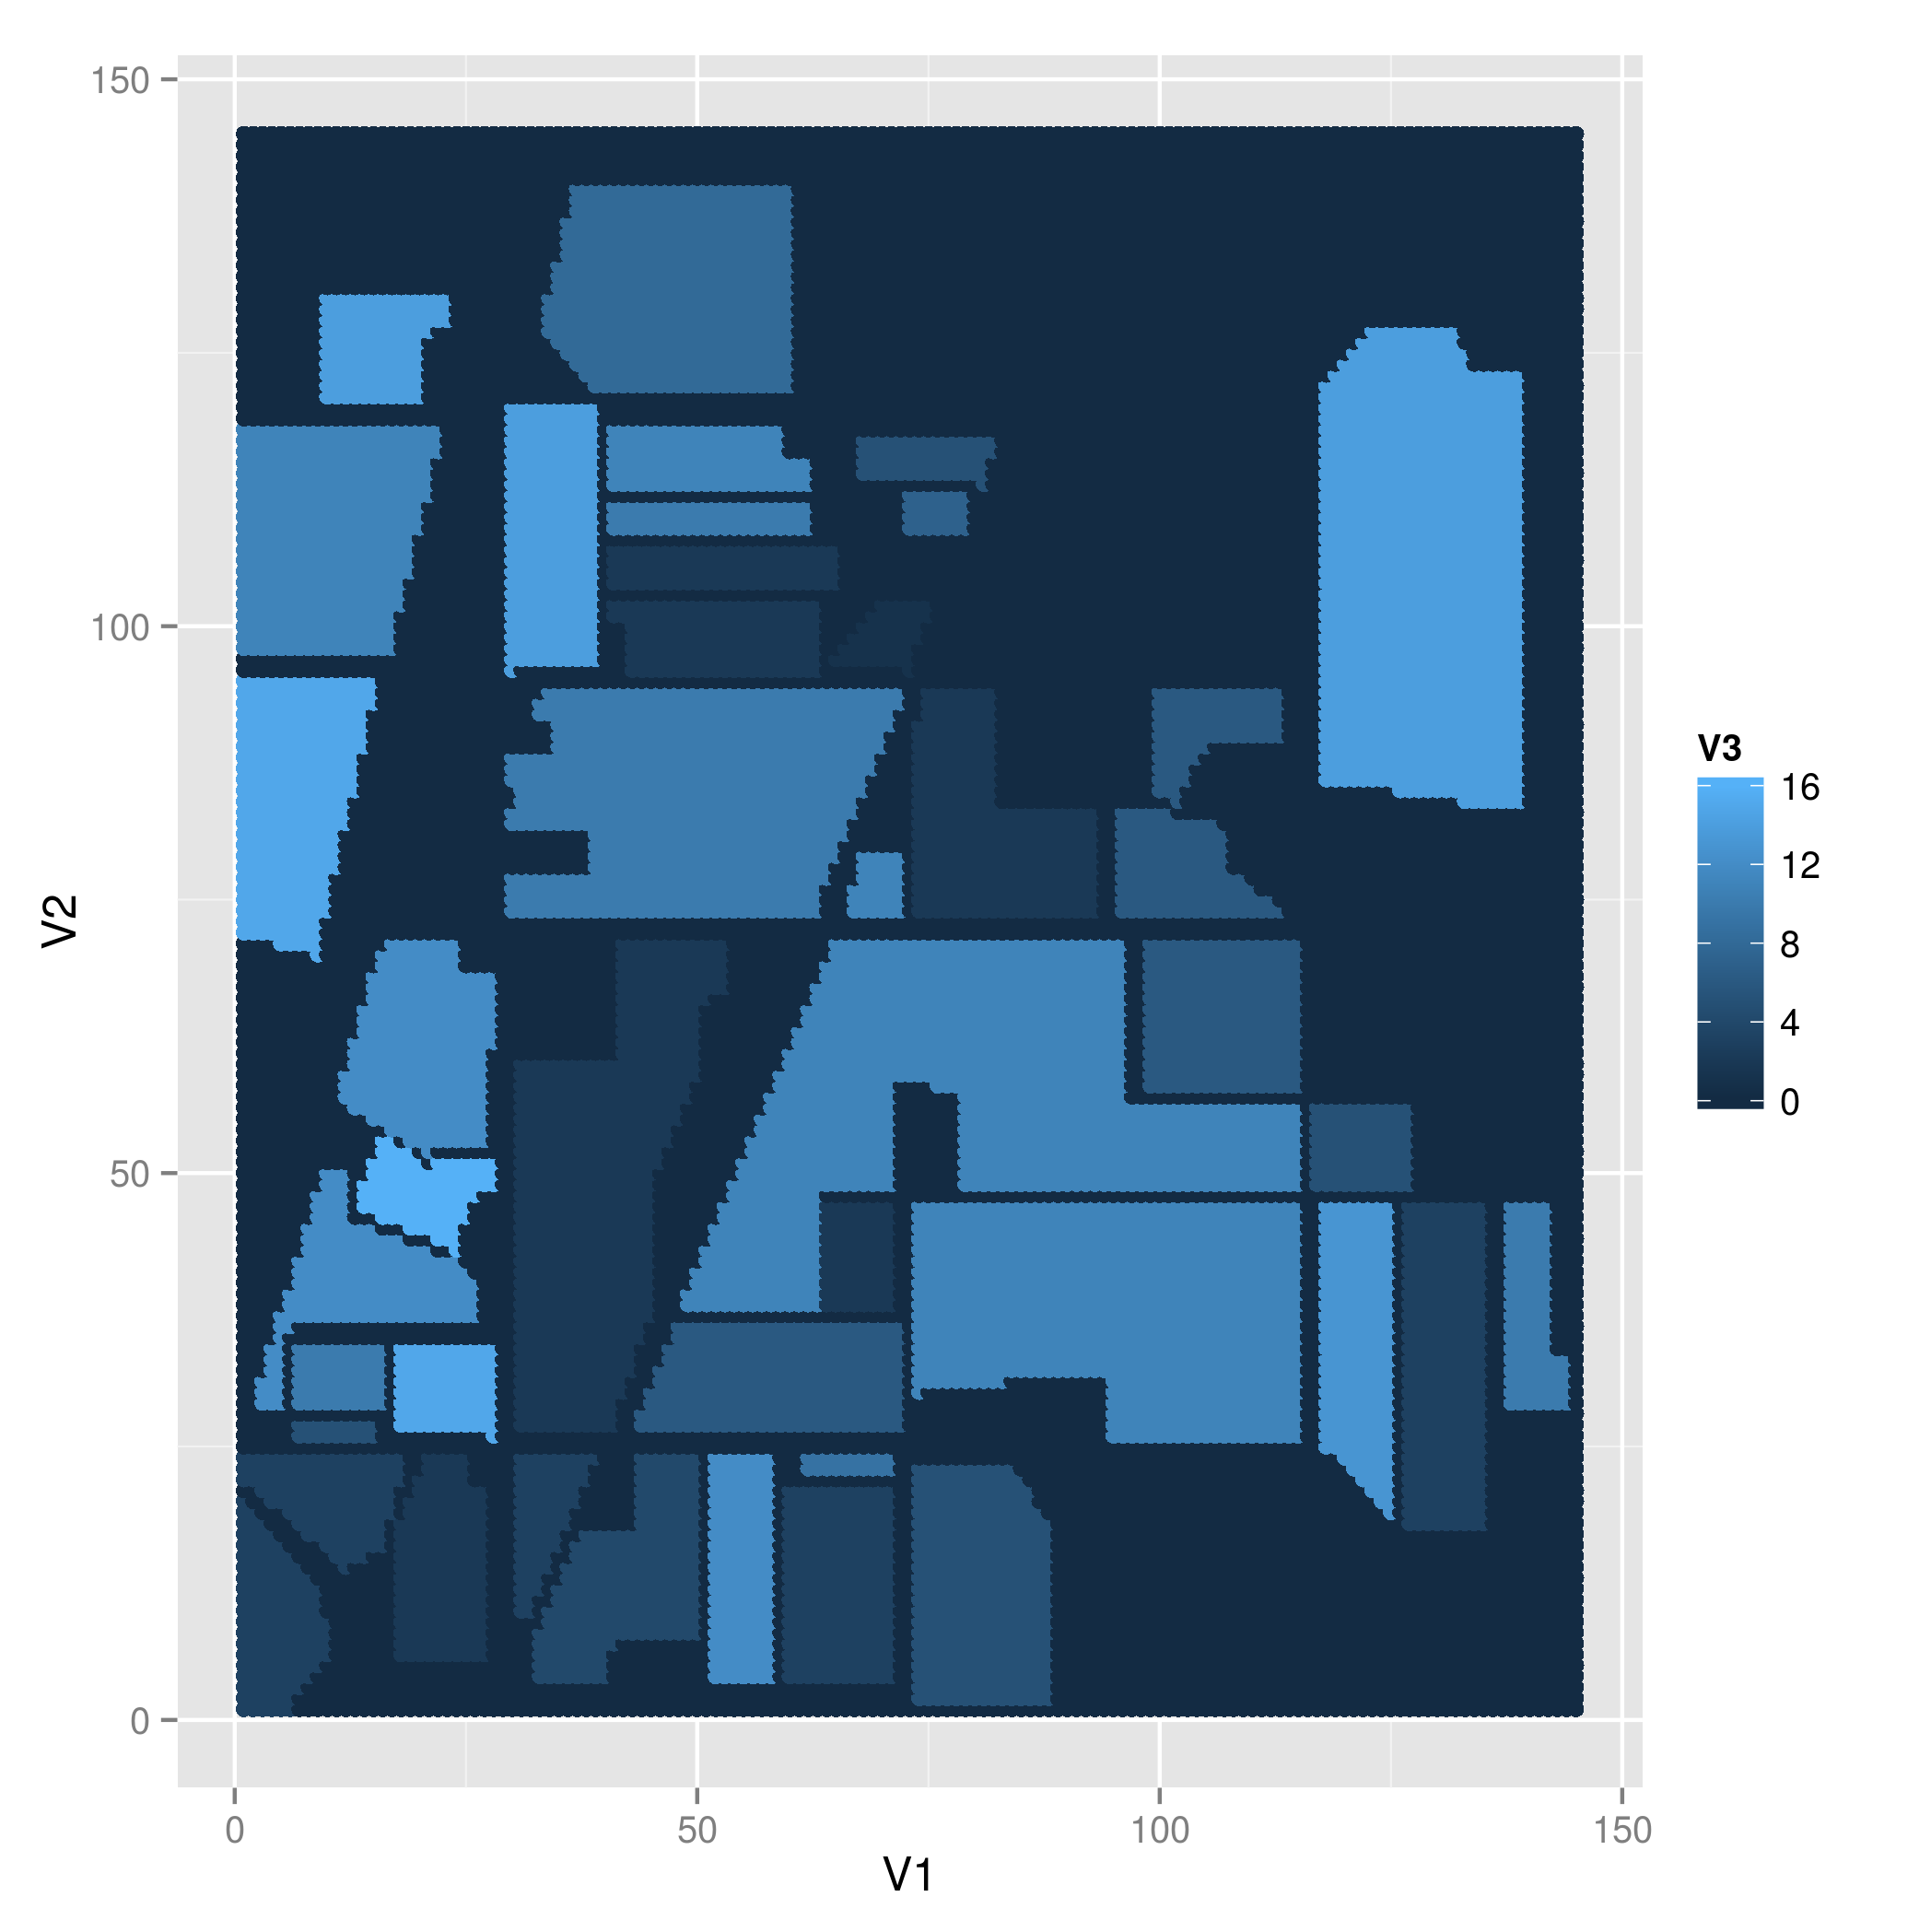
\includegraphics[width=0.38\textwidth]{../Presentation/gt.png}
\caption{Ground truth data}
\end{center}
\end{wrapfigure}

Overall, the ability to separate and classify each data point using every band was a success. The k-means clustering was able to roughly identify the different landtypes and shapes seen in the ground image. Noise was introduced because of the lack of spacial awareness in the K-means function. One possible noise reduction method would be to weight the spectra beforehand to rely more on the crisply defined images. As is, some data points were classified incorrectly simply because of their proximity to other high-noise points.

Given a training subset of 25\%, the soft-margin multiple SVM could predict approximately 83.5\% of the data accurately compared to the ground truth. This could be explained by the kernel which was used as well as the fact that the data was nonlinear.

For the principal component analysis, the data set was reduced and then examined either with weighting or without weighting. More than 90\% of the variance in the data could be explained by the first three principal components. By reducing the data set down from 21025 variables to 200, there is only a loss of about 10\% of information when only considering the first 3 of 200 variables. This disproportionate distribution of noise in the first few components allows for less noise and better dimensionality reduction. 
\section{Future Work}
Using both linear and nonlinear Gaussian models after preprocessing to separate the data would be less computationally expensive in comparison to k-means. More analysis on multiclass-SVM could lead to a higher accuracy in the separation of landtypes. Further dimensionality reduction would also be another solution to faster computations, but this could lead to higher inaccuracies or more loss in data.

Post processing using mathematical morphology may also reduce noise in the predicted values. Since farmland is generally solid, inorganic shapes, closing (or opening) the predicted groups may reduce the noise.

Noise reduction could also be approached by attempting to identify noisy spectra in the data. Some spectra appeared to contribute little to the model while including large amounts of noise. By reducing the influence of these less important spectra, we may improve the model.
\pagebreak
\section{Appendix}
\subsection{GitHub}
All code is available at \url{https://github.com/kycolton/drunken-secret-ninja}.
\subsection{Data Investigation}
\subsubsection{GIF of all Spectra}
\verbatiminput{../Code/gif_output.m}%a
\subsection{K-Means}
\subsubsection{Matlab}
\verbatiminput{../Code/km.m}%a
\subsubsection{R}
\verbatiminput{../Code/km.R}%a
\verbatiminput{../Code/plot_labels.R}
\subsection{SVM}
\verbatiminput{../Code/svm.R}
\subsection{PCA}
\verbatiminput{../Code/run_pca.m}
\end{document}